%% abtex2-modelo-trabalho-academico.tex, v-1.7.1 laurocesar
%% Copyright 2012-2013 by abnTeX2 group at http://abntex2.googlecode.com/ 
%%
%% This work may be distributed and/or modified under the
%% conditions of the LaTeX Project Public License, either version 1.3
%% of this license or (at your option) any later version.
%% The latest version of this license is in
%%   http://www.latex-project.org/lppl.txt
%% and version 1.3 or later is part of all distributions of LaTeX
%% version 2005/12/01 or later.
%%
%% This work has the LPPL maintenance status `maintained'.
%% 
%% The Current Maintainer of this work is the abnTeX2 team, led
%% by Lauro César Araujo. Further information are available on 
%% http://abntex2.googlecode.com/
%%
%% This work consists of the files abntex2-modelo-trabalho-academico.tex,
%% abntex2-modelo-include-comandos and abntex2-modelo-references.bib
%%

% ------------------------------------------------------------------------
% ------------------------------------------------------------------------
% abnTeX2: Modelo de Trabalho Academico (tese de doutorado, dissertacao de
% mestrado e trabalhos monograficos em geral) em conformidade com 
% ABNT NBR 14724:2011: Informacao e documentacao - Trabalhos academicos -
% Apresentacao
% ------------------------------------------------------------------------
% ------------------------------------------------------------------------


%%%%%%%%%%%%%%%%%%
%
% As alterações realizadas no leiaute original do abntex2 disponibilizado 
% no sharelatex adaptaram o leiaute do abntex2 aos requisitos mínimos
% para escrita de dissertações e teses customizadas para o 
% centro de informática da ufpe.
%
% Bruno Maciel <bifm@cin.ufpe.com> 20/10/2016
% Daniel Severo Estrázulas <dse@cin.ufpe.br> 19/10/2020
% Alterações realizadas para o template da biblioteca atualizado disponibilizado no site Versão 07.10.2020 (1.3) revisado pelas bibliotecárias do setor bibccen.pt@ufpe.br
%%%%%%%%%%%%%%%%%%%%%%%%%%%%%%%%%%%%%%%%%%%%%%%%%%%%%%%%%%%%%%%

%%%%%%%%%%%%%%%%%%
%
% As alterações realizadas no leiaute original do 
% MODELO LATEX ATUALIZADO BIBLIOTECA DO CCEN-UFPE - Versão 1.4 (16.10.2020) 
% disponibilizado no overleaf adaptando o leiaute do modelo do CIn aos requisitos 
% mínimos para escrita de dissertações e teses customizadas para a
% CESAR School.
%
% Tiago Barros <Tiago Barros> Março/2023
%%%%%%%%%%%%%%%%%%%%%%%%%%%%%%%%%%%%%%%%%%%%%%%%%%%%%%%%%%%%%%%

\documentclass[
	hidelinks,
	% -- opções da classe memoir --
	12pt,				% tamanho da fonte
	openright,			% capítulos começam em pág ímpar (insere página vazia caso preciso)
	oneside,			% para impressão em verso e anverso. Oposto a oneside
	a4paper,			% tamanho do papel. 
	% -- opções da classe abntex2 --
	chapter=TITLE,		% títulos de capítulos convertidos em letras maiúsculas
	section=TITLE,		% títulos de seções convertidos em letras maiúsculas
	%subsection=TITLE,	% títulos de subseções convertidos em letras maiúsculas
	%subsubsection=TITLE,% títulos de subsubseções convertidos em letras maiúsculas
	% -- opções do pacote babel --
	%english,			% idioma adicional para hifenização
	french,				% idioma adicional para hifenização
	spanish,			% idioma adicional para hifenização
%	brazil,				% o último idioma é o principal do documento
	english,
	brazil,
	]{abntex2/abntex2}
	\renewcommand{\baselinestretch}{1.5} %para customizar o espaço entre as linhas do texto
% --
% SETTINGS

\usepackage{abntex2/abntex2-cin-ufpe}

% \usepackage[noframe]{showframe}
% \usepackage{showframe}

%\overfullrule=4mm %para identificar onde existem os alertas de linhas grandes mal formatada pelo LaTex, basta comentar para não aparecer a barra lateral preta na linha em questão.

\renewcommand*\arraystretch{1.2} %para customizar o espaço entre as linhas das tabelas


\usepackage{pdfpages} %para incluir pdf como páginas


% ---
% PACOTES
% ---
\usepackage{float}
\usepackage{cmap}				% Mapear caracteres especiais no PDF
\usepackage{lmodern}			% Usa a fonte Latin Modern			
\usepackage[T1]{fontenc}		% Selecao de codigos de fonte.
\usepackage[utf8]{inputenc}		% Codificacao do documento (conversão automática dos acentos)
\usepackage{lastpage}			% Usado pela Ficha catalográfica
\usepackage{indentfirst}		% Indenta o primeiro parágrafo de cada seção.
%\usepackage{color}				% Controle das cores
\usepackage{graphicx}			% Inclusão de gráficos
\usepackage{lipsum}				% para geração de dummy text
\usepackage[versalete,alf,abnt-and-type=e,abnt-etal-list=0,abnt-etal-cite=3]{abntex2/abntex2cite} 
\usepackage{multirow}
\usepackage[section]{placeins}



% -----------------------------------------------------------
% lista de abreviaturas e siglas
% início
% -----------------------------------------------------------
% \usepackage[noredefwarn,acronym]{glossaries} %GLOSSÁRIO
\usepackage[acronym,nonumberlist,nogroupskip,noredefwarn]{glossaries}
% \usepackage{glossary-superragged}

\newcolumntype{L}[1]{>{\raggedright\let\newline\\\arraybackslash\hspace{0pt}}m{#1}}
\newcolumntype{C}[1]{>{\centering\let\newline\\\arraybackslash\hspace{0pt}}m{#1}}
\newcolumntype{R}[1]{>{\raggedleft\let\newline\\\arraybackslash\hspace{0pt}}m{#1}}

\newglossarystyle{modsuper}{%
  \glossarystyle{super}%
  \renewcommand{\glsgroupskip}{}
  
  % put the glossary in a longtable environment:
 \renewenvironment{theglossary}%
  {
    \begin{longtable}
        {L{0.2\textwidth}L{0.8\textwidth}}}%
    {\end{longtable}
  }%
}

% -----------------------------------------------------------
% lista de abreviaturas e siglas
% fim
% -----------------------------------------------------------


\usepackage{lscape} 
\usepackage{rotating} %rotates the figures, page
\usepackage{tikz}
\usepackage[section]{placeins}
\usepackage{setspace} 



% ----------------------------------------------------------
% PERSONALIZAÇÃO DE CORES
% ----------------------------------------------------------
\definecolor{blue}{RGB}{41,5,195}
\definecolor{gray}{rgb}{.4,.4,.4}
\definecolor{gray}{rgb}{.4,.4,.4}
\definecolor{pblue}{rgb}{0.13,0.13,1}
\definecolor{pgreen}{rgb}{0,0.5,0}
\definecolor{pred}{rgb}{0.9,0,0}
\definecolor{pgrey}{rgb}{0.46,0.45,0.48}
\definecolor{lightgray}{rgb}{0.95, 0.95, 0.96}
\definecolor{whitesmoke}{rgb}{0.96, 0.96, 0.96}
\definecolor{javared}{rgb}{0.6,0,0} % for strings
\definecolor{javagreen}{rgb}{0.25,0.5,0.35} % comments
\definecolor{javapurple}{rgb}{0.5,0,0.35} % keywords
\definecolor{javadocblue}{rgb}{0.25,0.35,0.75} % javadoc
\definecolor{meucinza}{rgb}{0.5, 0.5, 0.5}
%\definecolor{lightgray}{gray}{0.9}


% ----------------------------------------------------------
% PERSONALIZAÇÃO DO USUÁRIO
% ----------------------------------------------------------

% ----------------------------------------------------------
% DADOS DO TRABALHO - CAPA e FOLHA DE ROSTO
% Configure os dados do trabalho aqui
% ----------------------------------------------------------
%\newcommand{\instituicaoname}{Centro de Estudos e Sistemas Avançados do Recife - CESAR SCHOOL}
\newcommand{\programaname}{Programa de Doutorado Profissional em Engenharia de Software }
%\newcommand{\programaname}{Programa de Mestrado Profissional em Engenharia de Software }
\newcommand{\trabalhoname}{Tese de Doutorado }
%\newcommand{\trabalhoname}{Dissertação de Mestrado }

%\newcommand{\instituicaoname}{Recife Center for Advanved Studies and Systems - CESAR SCHOOL}
\newcommand{\instituicaoname}{CESAR SCHOOL}
%\newcommand{\programaname}{Professional Doctorate Program in Software Engineering }
%\newcommand{\programaname}{Professional Masters Program in Software Engineering }
%\newcommand{\trabalhoname}{Thesis }
%\newcommand{\trabalhoname}{Dissertation }

\titulo{\uppercase{\textbf{Título:} subtítulo}}
\autor{NOME COMPLETO DO (A) AUTOR (A)}
\local{Recife}
\data{\Year}
%\areaconcentracao{\textbf{\areacocentracaoname}: Texto Texto}
\orientador{\textbf{\orientadorname}: Texto Texto Texto}
\coorientador{\textbf{\coorientadorname}: Texto Texto Texto}

\instituicao{\textbf{\instituicaoname} }%\\ \programaname}
%\departamento{Centro de Texto}
\programa{Doutorado Profissional em Engenharia de Software}
\emailprograma{contato@cesar.school}
\siteprograma{https://cesar.school/mestrado-e-doutorado/ posgraduacao}

%\tipotrabalho{Trabalho de Conclusão de Curso}
%\tipotrabalho{Dissertação de Mestrado}
\tipotrabalho{\trabalhoname}

% O preambulo deve conter o tipo do trabalho, o objetivo, 
% o nome da instituição e a área de concentração 

%%%%%%%%%%%%%%%%%%%%%%%%%%%%%%%%%%%%%%%%%%%%%%%%%%%%%%
%% Protugues
%%%%%%%%%%%%
\preambulo{\trabalhoname apresentada ao \programaname do \instituicaoname, como requisito parcial para obtenção do grau de Doutor em Engenharia de Software.}

%\preambuloatadefesa{\trabalhoname apresentada ao \programaname do \instituicaoname, como requisito parcial para a obtenção do título de Doutor em Engenharia de Software em <dia> de <mes> de <ano>.}


%%%%%%%%%%%%%%%%%%%%%%%%%%%%%%%%%%%%%%%%%%%%%%%%%%%%%%
%% Ingles
%%%%%%%%%
%\preambulo{\trabalhoname presented to the \programaname at the \instituicaoname, as a partial requirement to obtain the degree of Doctor in Software Engineering.}

%\preambuloatadefesa{\trabalhoname presented to the \programaname at the \instituicaoname, as a partial requirement to obtain the degree of Doctor in Software Engineering at <month> <day>, <year>.}


\input{userlists}






% ----------------------------------------------------------
% COMPILA O ÍNDICE
% ----------------------------------------------------------
\makeindex
% ---


% ----------------------------------------------------------
% LISTA E ABREVIATURAS E SIGLAS
% ----------------------------------------------------------
%lista de siglas
\newacronym{MEC}{MEC}{Ministério da Educação}
\newacronym{UFPE}{UFPE}{Universidade Federal de Pernambuco}


\makenoidxglossaries
\renewcommand*{\glsseeformat}[3][\seename]{\textit{#1}  
\glsseelist{#2}}

\renewcommand*{\glspostdescription}{} % remove trailing dot
\renewcommand{\glsnamefont}[1]{\textbf{#1}}

\renewcommand{\familydefault}{\sfdefault}

% ----------------------------------------------------------
% GLOSSÁRIO
% ----------------------------------------------------------

\newglossaryentry{naive-bayes}
{
  name=\textit{Na{\"i}ve Bayes},
  description={},
  plural=\textit{Na{\"i}ve Bayes}
}

\newglossaryentry{hoeffding-tree}
{
  name=\textit{Hoeffding Tree},
  description={},
  plural=\textit{Hoeffding Trees}
}















\usepackage{pdfpages}
\usepackage{inconsolata}
\usepackage{listings}

\definecolor{cinza}{HTML}{FCF8F8}

% define formato e estilo dos elementos do tipo Codigo Fonte
\lstset{language=PHP,
basicstyle=\ttfamily\scriptsize,
%basicstyle=\ttfamily,
keywordstyle=\color{javapurple}\bfseries,
stringstyle=\color{pblue},
commentstyle=\color{javagreen},
morecomment=[s][\color{javadocblue}]{/**}{*/},
morecomment=[s][\color{gray}]{@}{\ },
numbers=left,
numberstyle=\tiny\color{black},
backgroundcolor=\color{cinza},
stepnumber=2,
numbersep=8pt,
xleftmargin=14pt,
tabsize=4,
showspaces=false,
showstringspaces=false,
breaklines=true,}

%%%%%%%%%%%%%%%%%%%%%%%%%%%%%%%%%%



\usepackage{adjustbox} % ajustar tabela ao tamanho da pagina


% ----------------------------------------------------------
% INÍCIO DO DOCUMENTO
% ----------------------------------------------------------
\begin{document}

\frenchspacing % Retira espaço extra obsoleto entre as frases.

\imprimircapa
\imprimirfolhaderosto*~
%a ficha deve ser passada pelo setor da biblioteca e sobrescrito no formato pdf

\includepdf[pages=-]{others/ficha.pdf}

%\newpage
%\input{others/ata_defesa}
%O MODELO de folha de aprovação encontra-se na pasta "others" no arquivo: MODELO_FOLHA_APROVACAO.docx
% Basta inserir as informações do seu trabalho e gerar um PDF com o mesmo nome, sobrescrevendo 
% MODELO_FOLHA_APROVACAO.pdf na pasta "others" que será incluido automaticamente no trbalho.
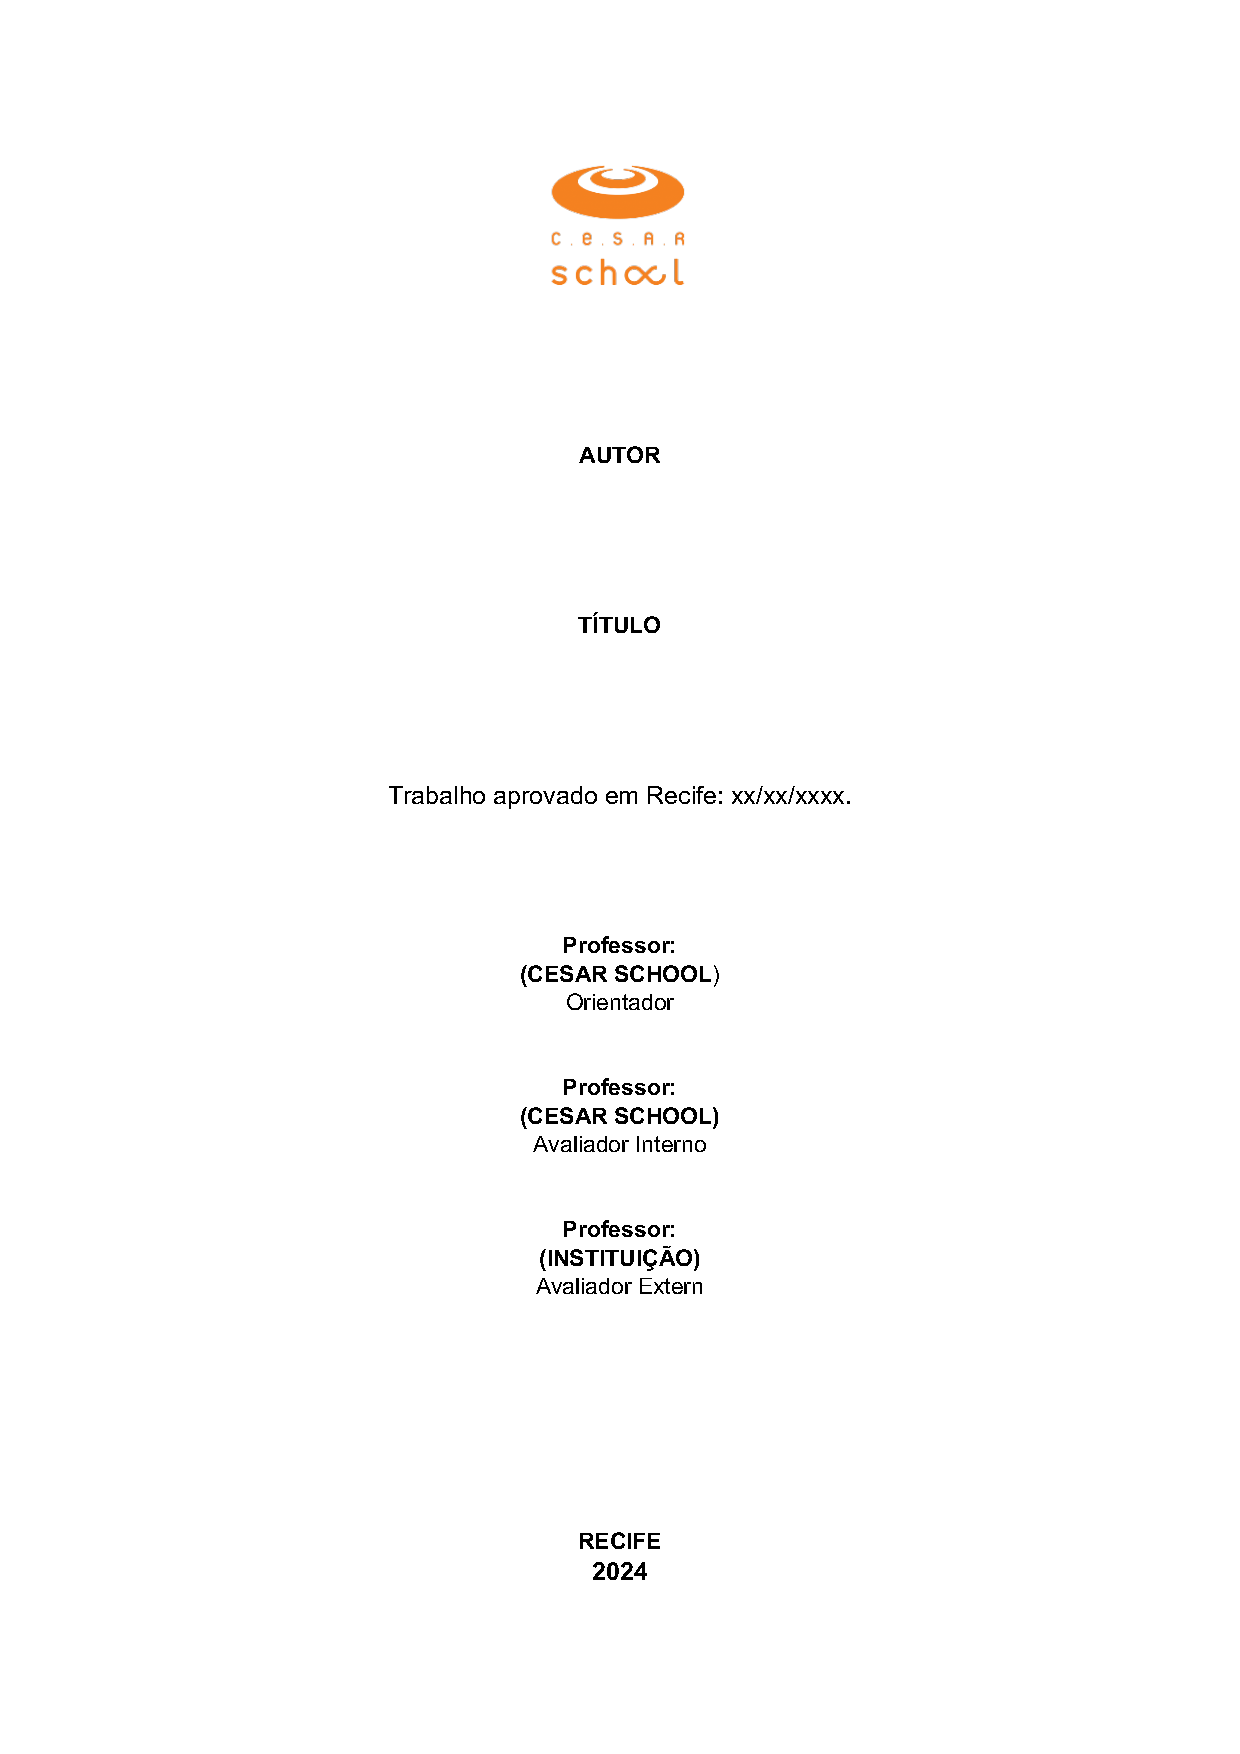
\includepdf[pages=-]{others/MODELO_FOLHA_APROVACAO}

% ----------------------------------------------------------
% DEDICATÓRIA
% ----------------------------------------------------------
\begin{dedicatoria}
   \vspace*{\fill}
%   \centering
  % \noindent
   %\textit{\lipsum[2]} 
   A Dedicatória é um elemento opcional do texto. Dedico este trabalho a texto texto texto texto texto texto texto texto texto texto texto texto texto texto texto texto texto texto texto texto texto texto texto texto texto texto texto texto texto texto texto texto texto texto texto texto texto texto texto texto texto. Texto texto texto texto texto texto texto texto texto texto texto texto texto texto texto texto texto texto texto texto texto texto texto texto texto texto texto texto texto texto texto texto texto texto texto texto texto texto texto texto texto texto.
   %\vspace*{\fill}
\end{dedicatoria}
% ---

% ----------------------------------------------------------
% AGRADECIMENTOS
% ----------------------------------------------------------
\begin{agradecimentos}
INÍCIO DO TEXTO DE AGRADECIMENTOS, ESTE É UM ELEMENTO OPCIONAL. Texto texto texto texto texto texto texto texto texto texto texto texto texto texto texto texto texto texto texto texto texto texto texto texto texto texto texto texto texto texto texto texto texto texto texto texto texto texto texto texto texto texto.

Texto texto texto texto texto texto texto texto texto texto texto texto texto texto texto texto texto texto texto texto texto texto texto texto texto texto texto texto texto texto texto texto texto texto texto texto texto texto texto texto texto texto.

Texto texto texto texto texto texto texto texto texto texto texto texto texto texto texto texto texto texto texto texto texto texto texto texto texto texto texto texto texto texto texto texto texto texto texto texto texto texto texto texto texto texto.

Texto texto texto texto texto texto texto texto texto texto texto texto texto texto texto texto texto texto texto texto texto texto texto texto texto texto texto texto texto texto texto texto texto texto texto texto texto texto texto texto texto texto.



\end{agradecimentos}


% ----------------------------------------------------------
% EPÍGRAFE

%Epígrafe: Elemento opcional e sem título em que o (a) autor (a) apresenta uma citação relacionada ao assunto tratado no trabalho. Deve ser elaborada conforme a ABNT-NBR 10520 (Citações). As citações de até três linhas devem estar entre aspas duplas e as citações com mais de três linhas devem ser destacadas com recuo de 4 cm da margem esquerda, com letra menor que a do texto e sem as aspas. A fonte da citação deve aparecer na lista de referências.
% ---------------------------------------------------------
\vspace*{10cm}
\begin{citacao}
Texto texto texto texto texto texto texto texto texto texto texto texto texto.Texto texto texto texto texto texto texto texto texto texto texto texto texto texto texto texto texto texto texto texto texto texto texto texto texto texto texto texto texto texto texto texto texto texto texto texto texto texto texto texto texto texto texto texto texto texto texto texto texto texto texto texto texto texto texto texto texto texto texto texto texto texto \cite{manualufpe2020}.
\end{citacao}

    \vspace*{5cm}
	
		''Texto texto texto texto texto texto texto texto texto texto texto texto texto texto texto texto texto texto texto texto texto texto texto texto texto.'' \cite[p. 4]{manualufpe2020}.
	
\newpage

% resumo em português
\begin{resumo}[Resumo] 
Texto de resumo em português, com 150 a 500 palavras. O resumo deve ter apenas 1 parágrafo, sem citações e sem recuo de texto na primeira linha. Também não pode haver quebra de linha. O resumo em portugues é necessário mesmo que o seu texto principal esteja em inglês. Texto texto texto texto texto texto texto texto texto texto texto texto texto texto texto texto texto texto texto texto texto texto texto texto texto texto texto texto texto texto texto texto texto texto texto texto texto texto texto texto texto texto texto texto texto texto texto texto texto texto texto texto texto texto texto texto texto texto texto texto texto texto texto texto texto texto texto texto texto texto texto texto texto texto texto texto texto texto texto texto texto texto texto texto texto texto texto texto texto texto texto texto texto texto texto texto texto texto texto texto texto texto texto. Texto texto texto texto texto texto texto texto texto texto texto texto texto texto texto texto texto texto texto texto texto texto texto texto texto texto texto texto texto texto texto texto texto texto texto texto texto texto texto texto texto texto texto texto texto texto texto texto texto texto texto texto texto texto texto texto texto texto texto texto texto texto texto texto texto texto texto texto texto texto texto texto texto texto texto texto texto texto texto texto texto texto texto texto texto texto texto texto texto texto texto texto texto texto texto texto texto texto texto texto texto texto texto. Texto texto texto texto texto texto texto texto texto texto texto texto texto texto texto texto texto texto texto texto texto texto texto texto texto texto texto texto texto texto texto texto texto texto texto texto texto texto texto texto texto texto texto texto texto texto texto texto texto texto texto texto texto texto texto texto texto texto texto texto texto texto texto texto texto texto texto texto texto texto texto texto texto texto texto texto texto texto texto texto texto texto texto texto texto texto texto texto texto texto texto texto texto texto texto texto texto texto texto texto texto texto texto. 
% \noindent %- o resumo deve ter apenas 1 parágrafo e sem recuo de texto na primeira linha, essa tag remove o recuo. Não pode haver quebra de linha.

 \vspace{\onelineskip}
    
 \noindent
 \textbf{Palavras-chave}: Palavras-chave; separadas; por; ponto; e; virgula.
\end{resumo}



% resumo em inglês
\begin{resumo}[Abstract]
\begin{otherlanguage*}{english}

 %\noindent
Abstract text in english, with 150 to 500 words. Must follow the same rules as the abstract in Portuguese. The abstract in english is necessary even if the main text is written in portuguese. Text text text text text text text text text text text text text text text text text text text text text text text text text text text text text text text text text text text text text text text text text text text text text text text text text text text text text text text text text text text text text text text text text text text text text text text text text text text text text text text text text text text text text text text text text text text text text text text text text text text. Text text text text text text text text text text text text text text text text text text text text text text text text text text text text text text text text text text text text text text text text text text text text text text text text text text text text text text text text text text text text text o text text text text text text text text text text text text text text text text text text text text text text text text text text text text text text text text text text text text text text. Text text text text text text text text text text text text text text text text text text text text text text text text text text text text text text text text text text text text text text text text text text text text text text text text text text text text text text text text text text text text text text text text text text text text text text text text text text text text text text text text text text text text text text text text text text text text text text text text text text text text text text text text text text text text text text text.



   \vspace{\onelineskip} 
 
   \noindent 
   \textbf{Keywords}: Keywords; separated; by; semicolon; Text; Text.
  \end{otherlanguage*}
 \end{resumo}



% ----------------------------------------------------------
% LISTA DE FIGURAS
% ----------------------------------------------------------
\pdfbookmark[0]{\listfigurename}{lof}
\listoffigures*
\cleardoublepage

% ----------------------------------------------------------
% LISTA DE GRAFICOS
% ----------------------------------------------------------
\pdfbookmark[0]{\listofgraficosname}{logr} % caso não tenha graficos, comente esta linha 
\listofgraficos* % caso não tenha graficos, comente esta linha 
\cleardoublepage


% ---
% LISTA DE CÓDIGOS FONTES
% ---

\pdfbookmark[0]{\lstlistingname}{lol} % caso não tenha quadros, comente esta linha 
\counterwithout{lstlisting}{chapter}



% Altera o nome padrão do rótulo usado no comando \autoref{}
\renewcommand{\lstlistingname}{Código Fonte}

% Altera o rótulo a ser usando no elemento pré-textual "Lista de código"
\renewcommand{\lstlistlistingname}{Lista de códigos}

% Configura a ``Lista de Códigos'' conforme as regras da ABNT (para abnTeX2)
\begingroup\makeatletter
\let\newcounter\@gobble\let\setcounter\@gobbletwo
  \globaldefs\@ne \let\c@loldepth\@ne
  \newlistof{listings}{lol}{\lstlistlistingname}
  \newlistentry{lstlisting}{lol}{0}
\endgroup

\renewcommand{\cftlstlistingaftersnum}{\hfill--\hfil}

\let\oldlstlistoflistings\lstlistoflistings
{
\let\oldnumberline\numberline
\newcommand{\algnumberline}[1]{Código Fonte~#1~\enspace--~\enspace}
\renewcommand{\numberline}{\algnumberline}

\begin{KeepFromToc}
\lstlistoflistings
\end{KeepFromToc}
}
\cleardoublepage

% ---
% LISTA DE QUADROS
% ---
\pdfbookmark[0]{\listofquadrosname}{loq} % caso não tenha quadros, comente esta linha 
\listofquadros* % caso não tenha quadros, comente esta linha 
\cleardoublepage



% ----------------------------------------------------------
% LISTA DE TABELAS
% ----------------------------------------------------------

\pdfbookmark[0]{\listtablename}{lot}
\listoftables*
\cleardoublepage


        
  
% ----------------------------------------------------------
% LISTA E ABREVIATURAS E SIGLAS
% ----------------------------------------------------------
\printglossary[type=\acronymtype,title={\listadesiglasname},nonumberlist]
\printglossaries
% compile uma vez com o comando \printglossaries e depois compile novamente com o comando \printglossaries comentado para as páginas glossário e siglas serem ocultadas.

% ----------------------------------------------------------
% LISTA E ABREVIATURAS E SIGLAS
% ----------------------------------------------------------
% \setglossarystyle{modsuper}
% \printnoidxglossary[style=modsuper,type=\acronymtype,title={\listadesiglasname},nonumberlist]
% \printglossary[style=super, type=\acronymtype]
\cleardoublepage



% ----------------------------------------------------------
% LISTA DE SIMBOLOS
% ----------------------------------------------------------



% ---

% ---
% inserir lista de símbolos
% ---
\begin{simbolos}
  \item[$ \gamma $] Letra grega Gama
  %\item[$ \Lambda $] Lambda
  %\item[$ \zeta $] Letra grega minúscula zeta
  \item[$ \in $] Pertence
%  \item[$ \infty$] Infinito
%  \item[$ \ge$] Maior ou Igual
  \item[$ \delta$] Delta
  \item[$ \theta$] Teta
  \item[$ \sigma$] Sigma
  \item[$ \mu$] Mi
  
\end{simbolos}
% ---




% ----------------------------------------------------------
%


% ---

% ---
% inserir lista de símbolos
% ---
\begin{simbolos}
  \item[$ \gamma $] Letra grega Gama
  %\item[$ \Lambda $] Lambda
  %\item[$ \zeta $] Letra grega minúscula zeta
  \item[$ \in $] Pertence
%  \item[$ \infty$] Infinito
%  \item[$ \ge$] Maior ou Igual
  \item[$ \delta$] Delta
  \item[$ \theta$] Teta
  \item[$ \sigma$] Sigma
  \item[$ \mu$] Mi
  
\end{simbolos}
% ---






% ----------------------------------------------------------
% SUMÁRIO
% ----------------------------------------------------------
\pdfbookmark[0]{\contentsname}{toc}
\tableofcontents*
% \begingroup\intoctrue
% \tableofcontents*
% \endgroup
\cleardoublepage

% \setcounter{page}{13}
\setcounter{tocdepth}{2}
\setcounter{table}{0}




% ----------------------------------------------------------
% ELEMENTOS TEXTUAIS
% ----------------------------------------------------------
\textual


% referencie todos os arquivos de capítulos aqui, fique a vontade para
% fazer a sua organização de diretórios

  % exemplo de organização interna de um capítulo separando por mais de um arquivo

  \chapter{Texto Texto Texto}
\label{chap:intro}


 Texto \textit{text} texto texto texto texto texto texto texto texto texto texto texto texto texto texto texto texto texto texto texto texto texto texto texto texto texto texto texto texto texto texto texto texto texto texto texto, no \gls{MEC}.

 Segundo \citeonline{manualufpe2020}, o \gls{MEC}, texto texto texto texto texto texto texto texto texto texto texto texto texto texto texto texto texto texto texto texto texto texto texto texto texto texto texto texto texto texto texto texto texto texto texto texto .
 
 \begin{citacao}
 Texto \textit{text} texto texto texto texto texto texto texto texto texto texto texto texto texto texto texto texto texto texto texto texto texto texto texto texto texto texto texto texto texto texto texto texto texto texto texto texto texto texto texto texto texto \cite{manualufpe2020}.  
 \end{citacao}


 
 

  \section{Texto Texto Texto}
\label{motivacao}

Texto texto texto texto texto texto texto texto texto texto texto texto texto texto texto texto texto texto texto texto texto texto texto texto texto texto texto texto texto texto texto texto texto texto texto texto, \textbf{exemplo} sigla \gls{UFPE}.

\input{images/captitulo1/figuraex}

Texto texto texto texto texto texto texto texto texto texto texto texto texto texto texto texto texto texto texto texto texto texto texto texto texto texto texto texto texto texto texto texto texto texto texto texto, conforme Figuras \ref{fig:figuraex} e Figuras \ref{fig:figuraex2} e também Grafico \ref{graph:grafico1}, continua no Capítulo \ref{chap:outrocapitulo}.


\input{images/captitulo1/figuraex2}

Texto texto texto texto texto texto texto texto texto texto texto texto texto texto texto texto texto texto texto texto texto texto texto texto texto texto texto texto texto texto texto texto texto texto texto texto texto texto texto texto texto texto texto texto texto texto texto texto texto texto texto texto texto texto texto texto texto texto texto texto texto texto texto texto texto texto texto texto texto texto texto texto texto texto texto texto texto texto texto texto texto \gls{UFPE}.

\begin{grafico}[ht!]
\centering

\caption{\textmd{Texto Texto Texto Texto Texto Texto Texto}}
\label{graph:grafico1}
\fcolorbox{gray}{white}{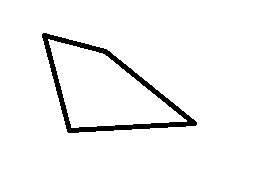
\includegraphics[width=0.80\textwidth]{images/captitulo1/figuraex.png}}

\fonteref{\citeauthor{manualufpe2020} (\citeyear{manualufpe2020})}
\end{grafico}

Texto texto texto texto texto texto texto texto texto texto texto texto texto texto texto texto texto texto texto texto texto texto texto texto texto texto texto \gls{UFPE} ver Diagrama \ref{diag:diagrama1}.

\begin{diagrama}[ht!]
\centering

\caption{\textmd{Texto do diagrama}}
\label{diag:diagrama1}
\fcolorbox{gray}{white}{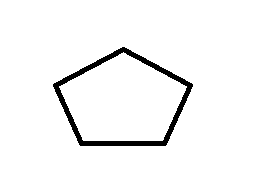
\includegraphics[width=0.80\textwidth]{images/captitulo1/figuraex2.png}}

\fonteadapt{\citeauthor{manualufpe2020} (\citeyear{manualufpe2020})}
\end{diagrama}
    
  
%  \input{chapters/introducao/problemahipotese.tex}
 
 \section{Texto Texto Texto}
\label{objetivos}
Texto texto texto texto texto texto texto texto texto texto texto texto texto texto texto texto texto texto texto texto texto texto texto texto texto texto texto texto texto texto texto texto texto texto texto texto.

Texto texto texto texto texto texto texto texto texto texto texto texto texto texto texto texto texto texto texto texto texto texto texto texto texto texto texto texto texto texto texto texto texto texto texto texto.

\subsection{Texto Texto Texto}
\label{sub:exemplonivel3}

Texto texto texto texto texto texto texto texto texto texto texto texto texto texto texto texto texto texto texto texto texto texto texto texto texto texto texto texto texto texto texto texto texto texto texto texto.

\subsubsection{Texto texto texto texto}
\label{subsub:exemplonivel4}

Texto texto texto texto texto texto texto texto texto texto texto texto texto texto texto texto texto texto texto texto texto texto texto texto texto texto texto texto texto texto texto texto texto texto texto texto.
      
% \input{chapters/introducao/organizacao.tex}

% .... 

  \chapter{Texto Texto Texto}
\label{chap:outrocapitulo}

Texto texto texto texto ''texto'' texto texto texto texto texto texto texto texto texto texto texto texto texto texto texto texto texto texto texto texto texto texto texto texto texto texto texto texto texto texto texto, confome Tabela \ref{tbl:tabelaex} e a Tabela \ref{tbl:tabelaex2}.

%exemplo de inputs, ideal para organização e troca de posicionamento futuro é ter um elemento por arquivo

%usar um gerador é uma opção https://www.tablesgenerator.com/
% observação, segundo a biblioteca tableas não podem ter nenhuma linha vertical

\begin{table}[ht]
\caption{Texto Texto Texto}
\label{tbl:tabelaex}
\centering
\rowcolors{1}{}{lightgray}
\begin{tabular}{p{6cm}p{9cm}}
\hline
\multicolumn{1}{c}{\textbf{Coluna A}} & \multicolumn{1}{c}{\textbf{Coluna B}}  \\
\hline     
\textbf{coluna1} & Texto Texto Texto Texto Texto Texto Texto Texto Texto Texto Texto Texto.
\\ 

coluna2 & Texto Texto Texto Texto Texto Texto Texto Texto Texto Texto Texto Texto.              
\\ 

coluna3 & Texto \textit{Texto} Texto Texto Texto Texto Texto Texto Texto Texto Texto Texto.     
\\ \hline

\end{tabular}

  \par\medskip\ABNTEXfontereduzida\selectfont\textbf{Fonte:} Elaborada pelo autor (2020) \par\medskip
\end{table}



%usar um gerador é uma opção https://www.tablesgenerator.com/
% observação, segundo a biblioteca tableas não podem ter nenhuma linha vertical

\begin{table}[ht]
\caption{Texto Texto Texto}
\label{tbl:tabelaex2}
\centering
\rowcolors{1}{}{lightgray}
\begin{tabular}{p{6cm}p{9cm}}
\hline
\multicolumn{1}{c}{\textbf{Coluna A}} & \multicolumn{1}{c}{\textbf{Coluna B}}  \\
\hline 
coluna1 & Texto Texto Texto Texto Texto Texto ''Texto'' Texto Texto Texto Texto Texto.
\\ 

coluna2 & Texto Texto Texto Texto Texto Texto Texto Texto Texto Texto Texto Texto.              
\\

coluna3 & Texto \textit{Texto} Texto Texto Texto Texto Texto Texto Texto Texto Texto Texto.     
\\ \hline

\end{tabular}

  \par\medskip\ABNTEXfontereduzida\selectfont\textbf{Fonte:} \citeauthor{manualufpe2020} (\citeyear{manualufpe2020}) \par\medskip
\end{table}


\section{Texto Texto}
\label{sec:section}

Texto texto texto texto ''texto'' texto texto texto texto texto texto texto texto texto texto texto texto texto texto texto texto texto texto texto texto texto texto texto texto texto texto texto texto texto texto texto \cite{gil2002elaborar}.


\section{Texto Texto}
\label{sec:outrasection}

Texto texto texto texto ''texto'' texto texto texto texto texto texto texto texto texto texto texto texto texto texto texto texto texto texto texto texto texto texto texto texto texto texto texto texto texto texto texto

\subsection{Texto Texto Texto}
\label{sub:outrasubsectiona}

Texto texto texto texto ''texto'' texto texto texto texto texto texto texto texto texto texto texto texto texto texto texto texto texto texto texto texto texto texto texto texto texto texto texto texto texto texto texto


\subsubsection{Texto Texto Texto Texto}
\label{subsub:outrasubsubsection}

Texto texto texto texto ''texto'' texto texto texto texto texto texto texto texto texto texto texto texto texto texto texto texto texto texto texto texto texto texto texto texto texto texto texto texto texto texto texto

\subsubsection{Texto Texto Texto Texto}
\label{subsub:outrasubsubsection2a}

Texto texto texto texto ''texto'' texto texto texto texto texto texto texto texto texto texto texto texto texto texto texto texto texto texto texto texto texto texto texto texto texto texto texto texto texto texto texto

%a organização fica a seu critério se preferir utilize inputs para cada seção, subseção etc...
%apenas um exemplo de subseção em arquivo para ser incluido
\subsection{Texto Texto Texto}
\label{sub:outrasubsection2}

Texto texto texto texto ''texto'' texto texto texto texto texto texto texto texto texto texto texto texto texto texto texto texto texto texto texto texto texto texto texto texto texto texto texto texto texto texto texto


\subsubsection{Texto Texto Texto Texto}
\label{subsub:outrasubsubsection2}

Texto texto texto texto ''texto'' texto texto texto texto texto texto texto texto texto texto texto texto texto texto texto texto texto texto texto texto texto texto texto texto texto texto texto texto texto texto texto

%apenas um exemplo de subseção em arquivo para ser incluido

\section{Texto Texto}
\label{sec:section3}

Texto texto texto texto ''texto'' texto texto texto texto texto texto texto texto texto texto texto texto texto texto texto texto texto texto texto texto texto texto texto texto texto texto texto texto texto texto texto
  
  \chapter{Texto Texto Texto}
%não se esqueça de definir uma label única para utilizar no comando \ref
\label{chap:metodologia}

Texto texto texto texto texto texto texto texto texto texto texto texto texto texto texto texto texto texto texto texto texto texto texto texto texto texto texto texto texto texto texto texto texto texto texto texto.

%exemplos de parágrafos com footnote
Texto texto texto texto texto texto texto texto texto texto texto texto texto texto texto texto texto texto texto texto texto texto texto texto texto texto texto texto texto texto texto texto texto texto texto texto \textit{Footnote} \footnote{Segundo \citeonline{manualufpe2020}, Exemplo de nota de rodapé.}.

\section{Texto Texto}
\label{sec:algumlabel}

Texto texto texto texto texto texto texto texto texto texto texto texto texto texto texto texto texto texto texto texto texto texto texto texto texto texto texto texto texto texto texto texto texto texto texto texto.

Texto texto texto texto texto texto texto texto texto texto texto texto texto texto texto texto texto texto texto texto texto texto texto texto texto texto texto texto texto texto texto texto texto texto texto texto \textit{Footnote} \footnote{Segundo \citeonline{manualufpe2020}, Exemplo de nota de rodapé 2.}.

%exemplo de código fonte, as configurações estão no arquivo packages.tex
\lstinputlisting[language=PHP, 
caption=Texto texto texto texto
,label=lst:exemplocodigo1]{chapters/trechos_codigo/funcoescatdinamicas.m}

\hspace{4cm}
\hfill
\begin{minipage}[t]{.65\textwidth}
\ABNTEXfontereduzida\selectfont\textbf{Fonte:} Elaborado pelo autor (2020) 
\end{minipage}


Texto texto texto texto texto texto texto texto texto texto texto texto texto texto texto texto texto texto texto texto texto texto texto texto texto texto texto texto texto texto texto texto texto texto texto texto, referente ao Código Fonte \ref{lst:exemplocodigo1} função \texttt{nome\_funcao}.

\subsection{Texto Texto Texto}
\label{subsec:algumlabel}

Texto texto texto texto texto texto texto texto texto texto texto texto texto texto texto texto texto texto texto texto texto texto texto texto texto texto texto texto texto texto texto texto texto texto texto texto.

\section{Texto Texto}
\label{sec:algumlabel2}
%exemplo de quadro
Texto texto texto texto texto texto texto texto texto texto texto texto texto texto texto texto texto texto texto texto texto texto texto texto texto texto texto texto texto texto texto texto texto texto texto texto, ver Quadro \ref{quad:exemplo_de_quadro}.

%a diferença do quadro pra tabela é que o quadro tem linhas verticais
\begin{quadro}
\caption{Texto texto texto texto texto}
\label{quad:exemplo_de_quadro}
\centering
\begin{tabular}{|lllll|}
\cline{1-5}
A& B &  C& D &E  \\ \cline{1-5}
\multirow{3}{*}{1}  & 2 &  3& 4& 5 \\
 &  2 &  3& 4& 5  \\
 &  2 &  3& 4& 5 \\
 \cline{1-5}
\end{tabular}
  \par\medskip\ABNTEXfontereduzida\selectfont\textbf{Fonte:} Elaborada pelo autor (2020) \par\medskip
\end{quadro}


\subsection{Texto Texto Texto}
\label{subsec:algumlabel2}
Texto texto texto texto texto texto texto texto texto texto texto texto texto texto texto texto texto texto texto texto texto texto texto texto texto texto texto texto texto texto texto texto texto texto texto texto.

\subsection{Texto Texto Texto}
\label{subsec:algumlabel3}

Texto texto texto texto texto texto texto texto texto texto texto texto texto texto texto texto texto texto texto texto texto texto texto texto texto texto texto texto texto texto texto texto texto texto texto texto.


  \chapter{Texto Texto Texto}
\label{chap:capitulo1}

Texto texto texto texto texto texto texto texto texto texto texto texto texto texto texto texto texto texto texto texto texto texto texto texto texto texto texto texto texto texto texto texto texto texto texto texto.


\lstinputlisting[language=Java, 
caption=Texto texto texto texto
,label=lst:exemplocodigo2]{chapters/trechos_codigo/java.m}
\hfill
\begin{minipage}[t]{.65\textwidth}
\ABNTEXfontereduzida\selectfont\textbf{Fonte:} \citeauthor{universidadejava2020}  (\citeyear{universidadejava2020}) 
\end{minipage}




\section{Texto Texto Texto}
\label{sec:label}
Texto texto texto texto texto texto texto texto texto texto texto texto texto texto texto texto texto texto texto texto texto texto texto texto texto texto texto texto texto texto texto texto texto texto texto texto, ver Capítulo \ref{chap:metodologia}, Seção \ref{sec:algumlabel}.

Texto texto texto texto texto texto texto texto texto texto texto texto texto texto texto texto texto texto texto texto texto texto texto texto texto texto texto texto texto texto texto texto texto texto texto texto (Código Fonte \ref{lst:exemplocodigo2}).


\section{Texto Texto}
\label{sec:outralabel}

Texto texto texto texto texto texto texto texto texto texto texto texto texto texto texto texto texto texto texto texto texto texto texto texto texto texto texto texto texto texto texto texto texto texto texto texto.



\bookmarksetup{startatroot}% 


% ----------------------------------------------------------
% ELEMENTOS PÓS-TEXTUAIS
% ----------------------------------------------------------
\postextual


% ----------------------------------------------------------
% Referências bibliográficas
% ----------------------------------------------------------
%\bibliographystyle{abntexalfenglish} %caso seja em inglês, retire o comentário desta linha

% \renewcommand{\bibname}{REFER\^ENCIAS}
%\renewcommand{\bibname}{Bibliography}
% \addbibresource{sample.bib}
\bibliography{references2}


% ----------------------------------------------------------
% Apêndices
% ----------------------------------------------------------


% ----------------------
% força para que não exiba subtítulos em apêndices no sumário
% -----------------------

\begin{apendicesenv}
\addtocontents{toc}{\protect\setcounter{tocdepth}{1}}
\makeatletter
\addtocontents{toc}{%
  \begingroup
  \let\protect\l@chapter\protect\l@section
  \let\protect\l@section\protect\l@subsection
}
\makeatother

% Imprime uma página indicando o início dos apêndices
% \partapendices

%coloca o identificador do anexo/apendice somente na primeira página
%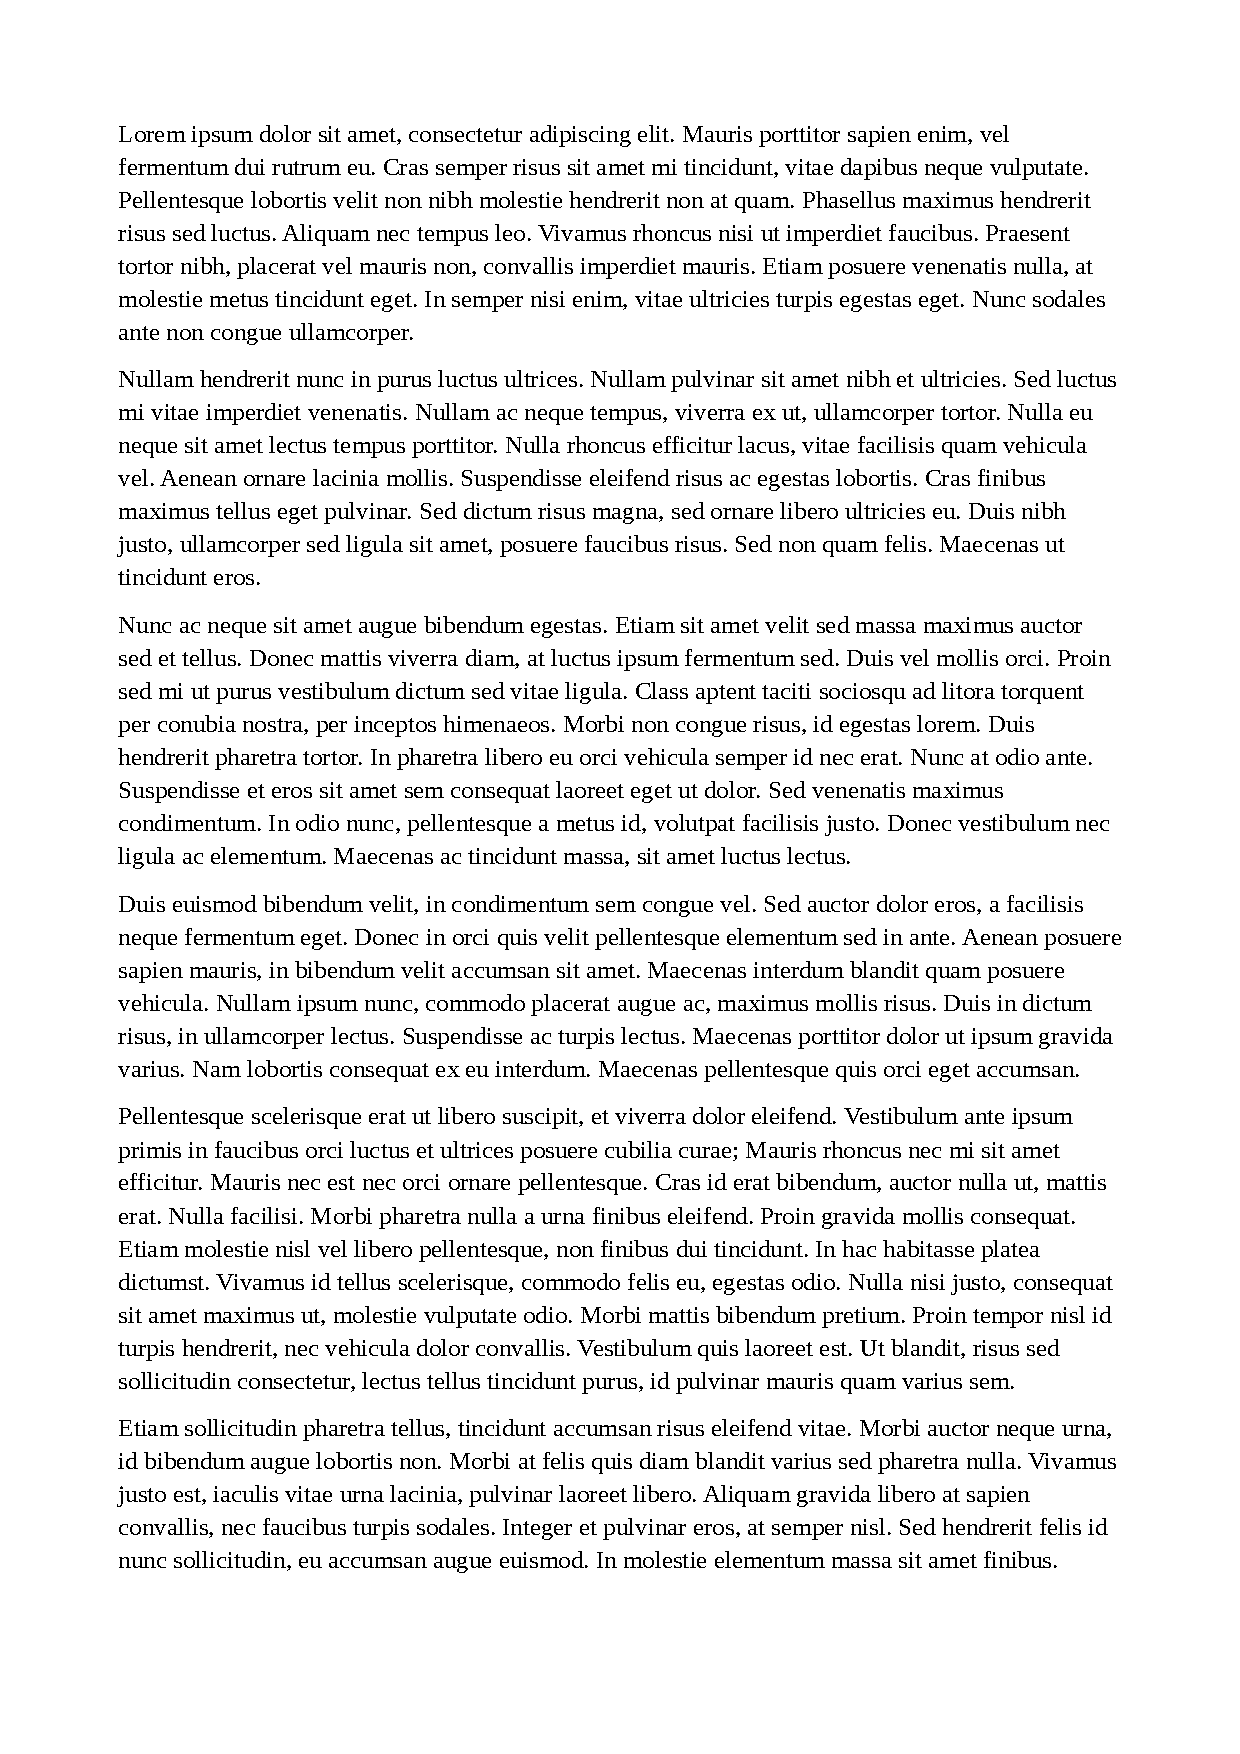
\includepdf[pages={1},scale=0.8,pagecommand=\chapter{Texto Texto Texto Texto}\label{apen:apendiceA}]{appendix/apendiceA}
%\includepdf[pages={2-},scale=0.80,pagecommand={}]{appendix/apendiceA}

\chapter{Titulo do Apendice A}\label{apen:apendiceA}

TEXTO TEXTO TEXTO TEXTO TEXTO TEXTO TEXTO TEXTO TEXTO TEXTO TEXTO TEXTO TEXTO TEXTO TEXTO TEXTO TEXTO TEXTO TEXTO TEXTO TEXTO TEXTO TEXTO TEXTO TEXTO TEXTO TEXTO TEXTO TEXTO TEXTO TEXTO TEXTO TEXTO TEXTO TEXTO TEXTO TEXTO TEXTO TEXTO TEXTO 
TEXTO TEXTO TEXTO TEXTO TEXTO TEXTO TEXTO TEXTO TEXTO TEXTO TEXTO TEXTO TEXTO TEXTO TEXTO TEXTO TEXTO TEXTO TEXTO TEXTO TEXTO TEXTO TEXTO TEXTO TEXTO TEXTO TEXTO TEXTO TEXTO TEXTO TEXTO TEXTO TEXTO TEXTO TEXTO TEXTO TEXTO TEXTO TEXTO TEXTO 
TEXTO TEXTO TEXTO TEXTO TEXTO TEXTO TEXTO TEXTO TEXTO TEXTO TEXTO TEXTO TEXTO TEXTO TEXTO TEXTO TEXTO TEXTO TEXTO TEXTO TEXTO TEXTO TEXTO TEXTO TEXTO TEXTO TEXTO TEXTO TEXTO TEXTO TEXTO TEXTO TEXTO TEXTO TEXTO TEXTO TEXTO TEXTO TEXTO TEXTO 
TEXTO TEXTO TEXTO TEXTO TEXTO TEXTO TEXTO TEXTO TEXTO TEXTO TEXTO TEXTO TEXTO TEXTO TEXTO TEXTO TEXTO TEXTO TEXTO TEXTO TEXTO TEXTO TEXTO TEXTO TEXTO TEXTO TEXTO TEXTO TEXTO TEXTO TEXTO TEXTO TEXTO TEXTO TEXTO TEXTO TEXTO TEXTO TEXTO TEXTO 
TEXTO TEXTO TEXTO TEXTO TEXTO TEXTO TEXTO TEXTO TEXTO TEXTO TEXTO TEXTO TEXTO TEXTO TEXTO TEXTO TEXTO TEXTO TEXTO TEXTO TEXTO TEXTO TEXTO TEXTO TEXTO TEXTO TEXTO TEXTO TEXTO TEXTO TEXTO TEXTO TEXTO TEXTO TEXTO TEXTO TEXTO TEXTO TEXTO TEXTO 
TEXTO TEXTO TEXTO TEXTO TEXTO TEXTO TEXTO TEXTO TEXTO TEXTO TEXTO TEXTO TEXTO TEXTO TEXTO TEXTO TEXTO TEXTO TEXTO TEXTO TEXTO TEXTO TEXTO TEXTO TEXTO TEXTO TEXTO TEXTO TEXTO TEXTO TEXTO TEXTO TEXTO TEXTO TEXTO TEXTO TEXTO TEXTO TEXTO TEXTO 

\section{Section 1 - A}

TEXTO TEXTO TEXTO TEXTO TEXTO TEXTO TEXTO TEXTO TEXTO TEXTO TEXTO TEXTO TEXTO TEXTO TEXTO TEXTO TEXTO TEXTO TEXTO TEXTO 
TEXTO TEXTO TEXTO TEXTO TEXTO TEXTO TEXTO TEXTO TEXTO TEXTO TEXTO TEXTO TEXTO TEXTO TEXTO TEXTO TEXTO TEXTO TEXTO TEXTO TEXTO TEXTO TEXTO TEXTO TEXTO TEXTO TEXTO TEXTO TEXTO TEXTO TEXTO TEXTO TEXTO TEXTO TEXTO TEXTO TEXTO TEXTO TEXTO TEXTO 
TEXTO TEXTO TEXTO TEXTO TEXTO TEXTO TEXTO TEXTO TEXTO TEXTO TEXTO TEXTO TEXTO TEXTO TEXTO TEXTO TEXTO TEXTO TEXTO TEXTO TEXTO TEXTO TEXTO TEXTO TEXTO TEXTO TEXTO TEXTO TEXTO TEXTO TEXTO TEXTO TEXTO TEXTO TEXTO TEXTO TEXTO TEXTO TEXTO TEXTO 
TEXTO TEXTO TEXTO TEXTO TEXTO TEXTO TEXTO TEXTO TEXTO TEXTO TEXTO TEXTO TEXTO TEXTO TEXTO TEXTO TEXTO TEXTO TEXTO TEXTO 
TEXTO TEXTO TEXTO TEXTO TEXTO TEXTO TEXTO TEXTO TEXTO TEXTO TEXTO TEXTO TEXTO TEXTO TEXTO TEXTO TEXTO TEXTO TEXTO TEXTO TEXTO TEXTO TEXTO TEXTO TEXTO TEXTO TEXTO TEXTO TEXTO TEXTO TEXTO TEXTO TEXTO TEXTO TEXTO TEXTO TEXTO TEXTO TEXTO TEXTO 
TEXTO TEXTO TEXTO TEXTO TEXTO TEXTO TEXTO TEXTO TEXTO TEXTO TEXTO TEXTO TEXTO TEXTO TEXTO TEXTO TEXTO TEXTO TEXTO TEXTO TEXTO TEXTO TEXTO TEXTO TEXTO TEXTO TEXTO TEXTO TEXTO TEXTO TEXTO TEXTO TEXTO TEXTO TEXTO TEXTO TEXTO TEXTO TEXTO TEXTO 

\subsection{Section 1.1 - A}

TEXTO TEXTO TEXTO TEXTO TEXTO TEXTO TEXTO TEXTO TEXTO TEXTO TEXTO TEXTO TEXTO TEXTO TEXTO TEXTO TEXTO TEXTO TEXTO TEXTO 
TEXTO TEXTO TEXTO TEXTO TEXTO TEXTO TEXTO TEXTO TEXTO TEXTO TEXTO TEXTO TEXTO TEXTO TEXTO TEXTO TEXTO TEXTO TEXTO TEXTO TEXTO TEXTO TEXTO TEXTO TEXTO TEXTO TEXTO TEXTO TEXTO TEXTO TEXTO TEXTO TEXTO TEXTO TEXTO TEXTO TEXTO TEXTO TEXTO TEXTO 
TEXTO TEXTO TEXTO TEXTO TEXTO TEXTO TEXTO TEXTO TEXTO TEXTO TEXTO TEXTO TEXTO TEXTO TEXTO TEXTO TEXTO TEXTO TEXTO TEXTO TEXTO TEXTO TEXTO TEXTO TEXTO TEXTO TEXTO TEXTO TEXTO TEXTO TEXTO TEXTO TEXTO TEXTO TEXTO TEXTO TEXTO TEXTO TEXTO TEXTO 
TEXTO TEXTO TEXTO TEXTO TEXTO TEXTO TEXTO TEXTO TEXTO TEXTO TEXTO TEXTO TEXTO TEXTO TEXTO TEXTO TEXTO TEXTO TEXTO TEXTO 
TEXTO TEXTO TEXTO TEXTO TEXTO TEXTO TEXTO TEXTO TEXTO TEXTO TEXTO TEXTO TEXTO TEXTO TEXTO TEXTO TEXTO TEXTO TEXTO TEXTO TEXTO TEXTO TEXTO TEXTO TEXTO TEXTO TEXTO TEXTO TEXTO TEXTO TEXTO TEXTO TEXTO TEXTO TEXTO TEXTO TEXTO TEXTO TEXTO TEXTO 
TEXTO TEXTO TEXTO TEXTO TEXTO TEXTO TEXTO TEXTO TEXTO TEXTO TEXTO TEXTO TEXTO TEXTO TEXTO TEXTO TEXTO TEXTO TEXTO TEXTO TEXTO TEXTO TEXTO TEXTO TEXTO TEXTO TEXTO TEXTO TEXTO TEXTO TEXTO TEXTO TEXTO TEXTO TEXTO TEXTO TEXTO TEXTO TEXTO TEXTO 


%coloca o identificador do anexo/apendice somente na primeira página
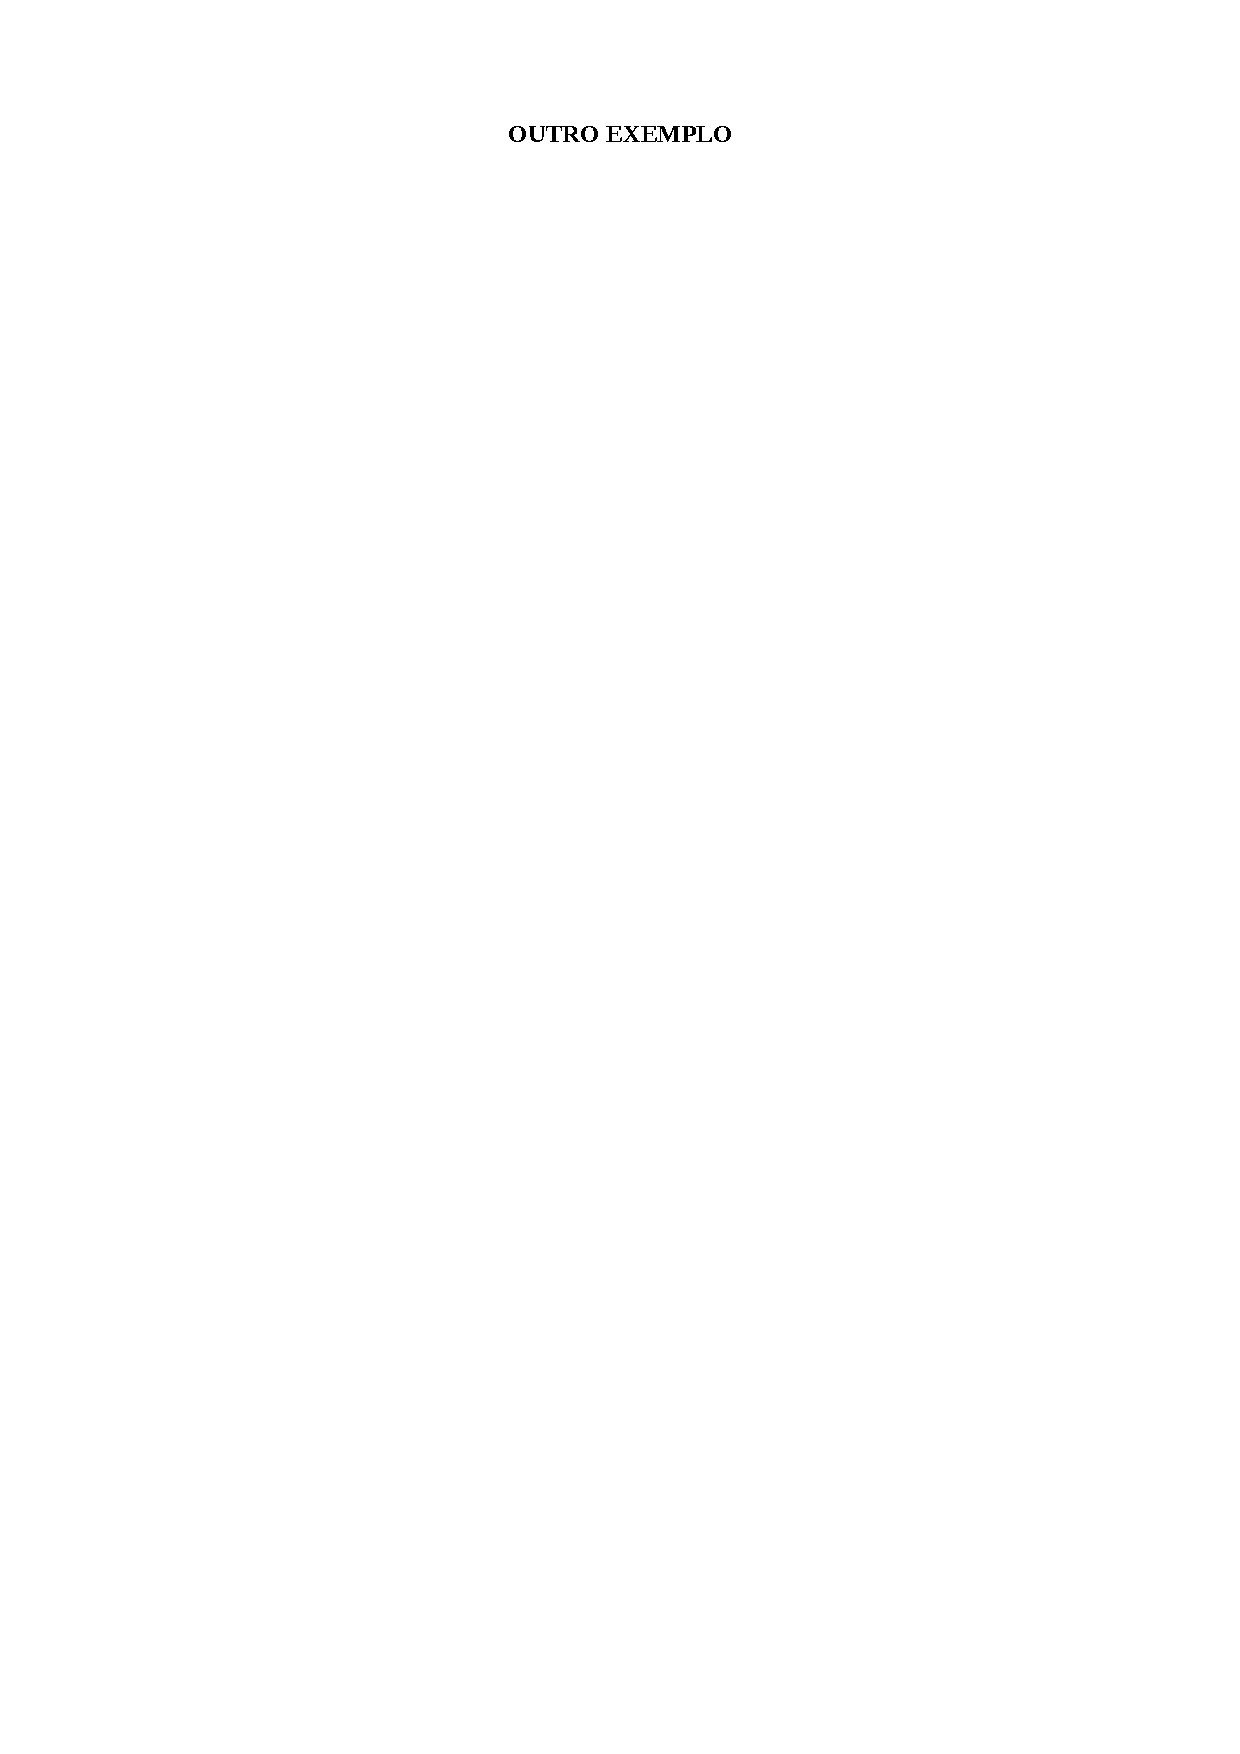
\includepdf[pages={1},scale=0.80,pagecommand=\chapter{Texto Texto Texto}\label{apen:apendiceB}]{appendix/apendiceB}


%coloca o identificador do anexo/apendice somente na primeira página
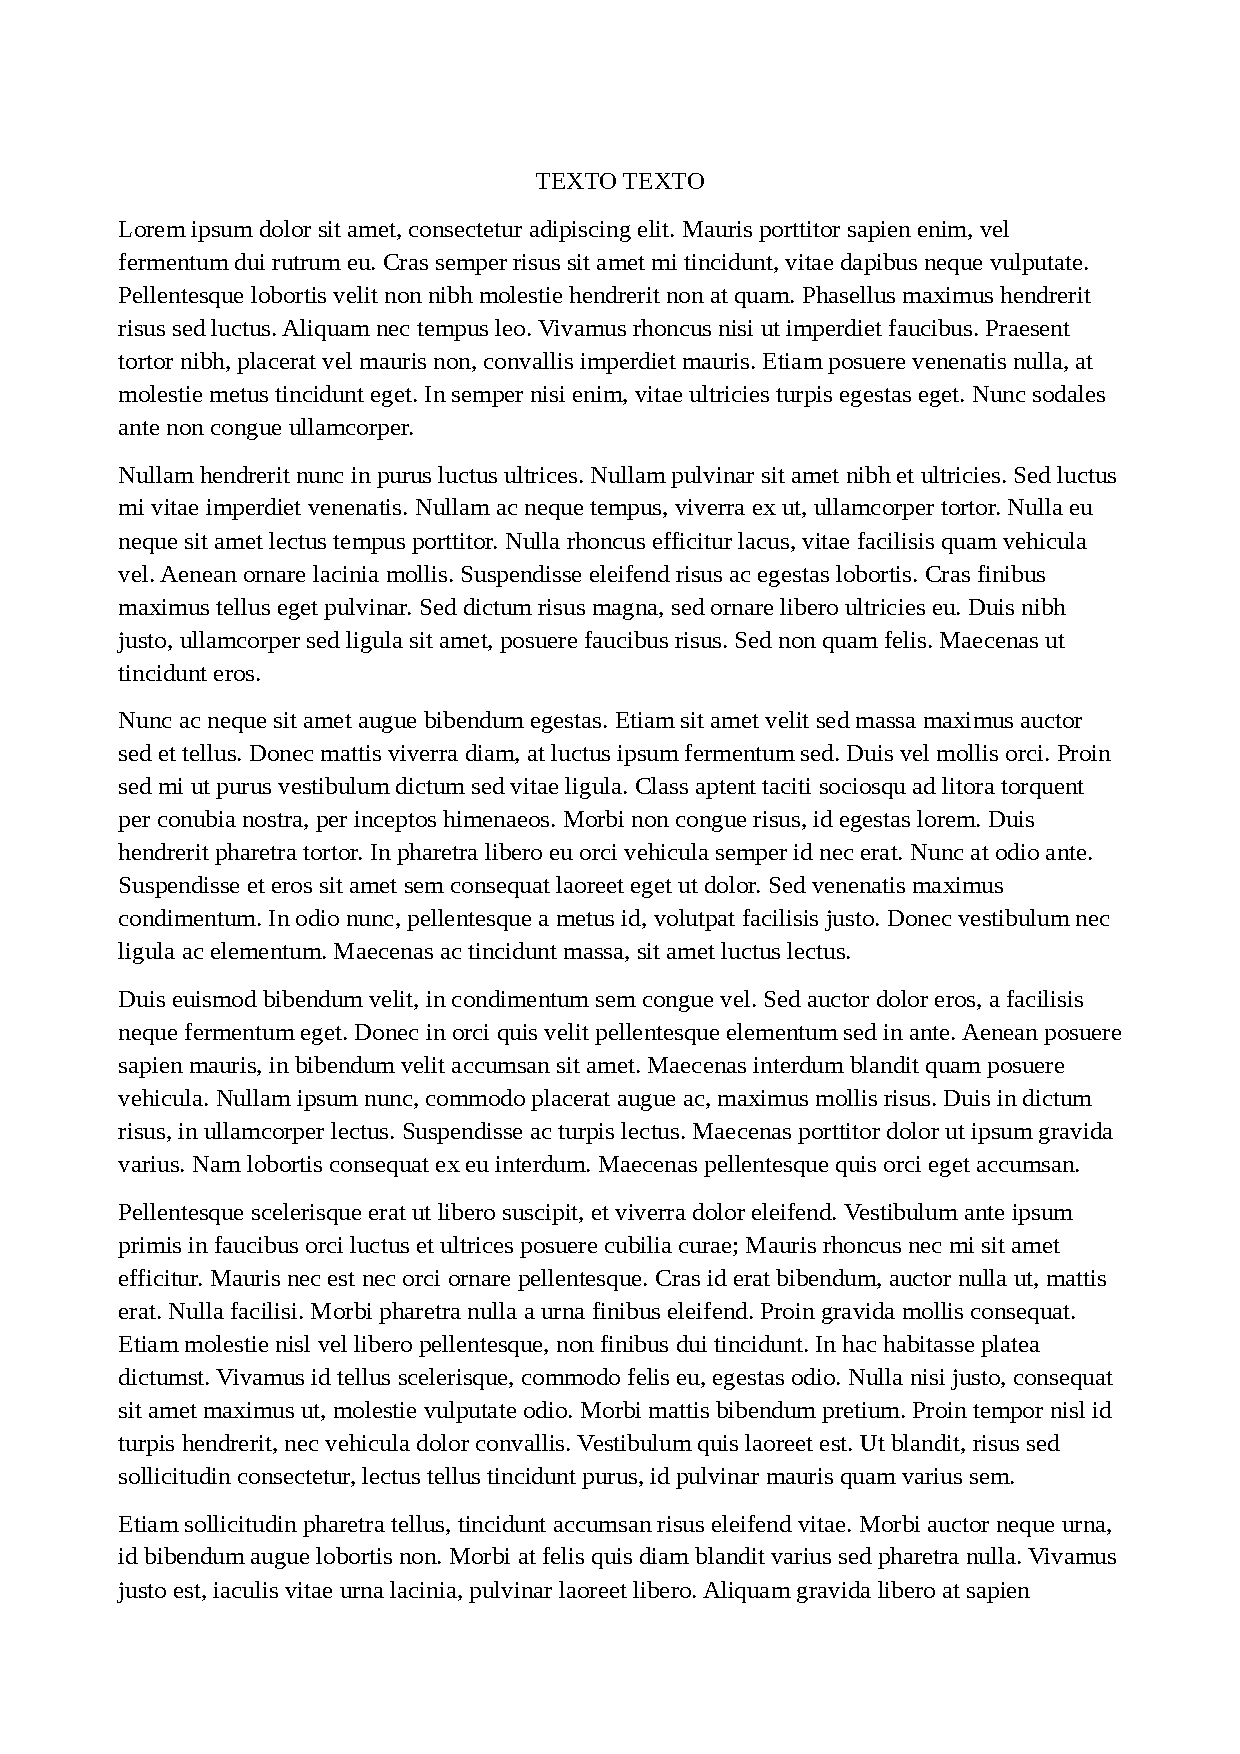
\includepdf[pages={1},scale=0.80,pagecommand=\chapter{Texto Texto}\label{apen:apendiceC}]{appendix/apendiceC}
\includepdf[pages={2},scale=0.80,pagecommand={}]{appendix/apendiceC}


\addtocontents{toc}{\endgroup}
\end{apendicesenv}




% ----------------------------------------------------------
% Anexos
% ----------------------------------------------------------

% ----------------------
% força para que não exiba subtítulos em apêndices no sumário
% -----------------------

\begin{anexosenv}
\addtocontents{toc}{\protect\setcounter{tocdepth}{1}}
\makeatletter
\addtocontents{toc}{%
  \begingroup
  \let\protect\l@chapter\protect\l@section
  \let\protect\l@section\protect\l@subsection
}
\makeatother
% Imprime uma página indicando o início dos apêndices
% \partapendices

%coloca o identificador do anexo/apendice somente na primeira página
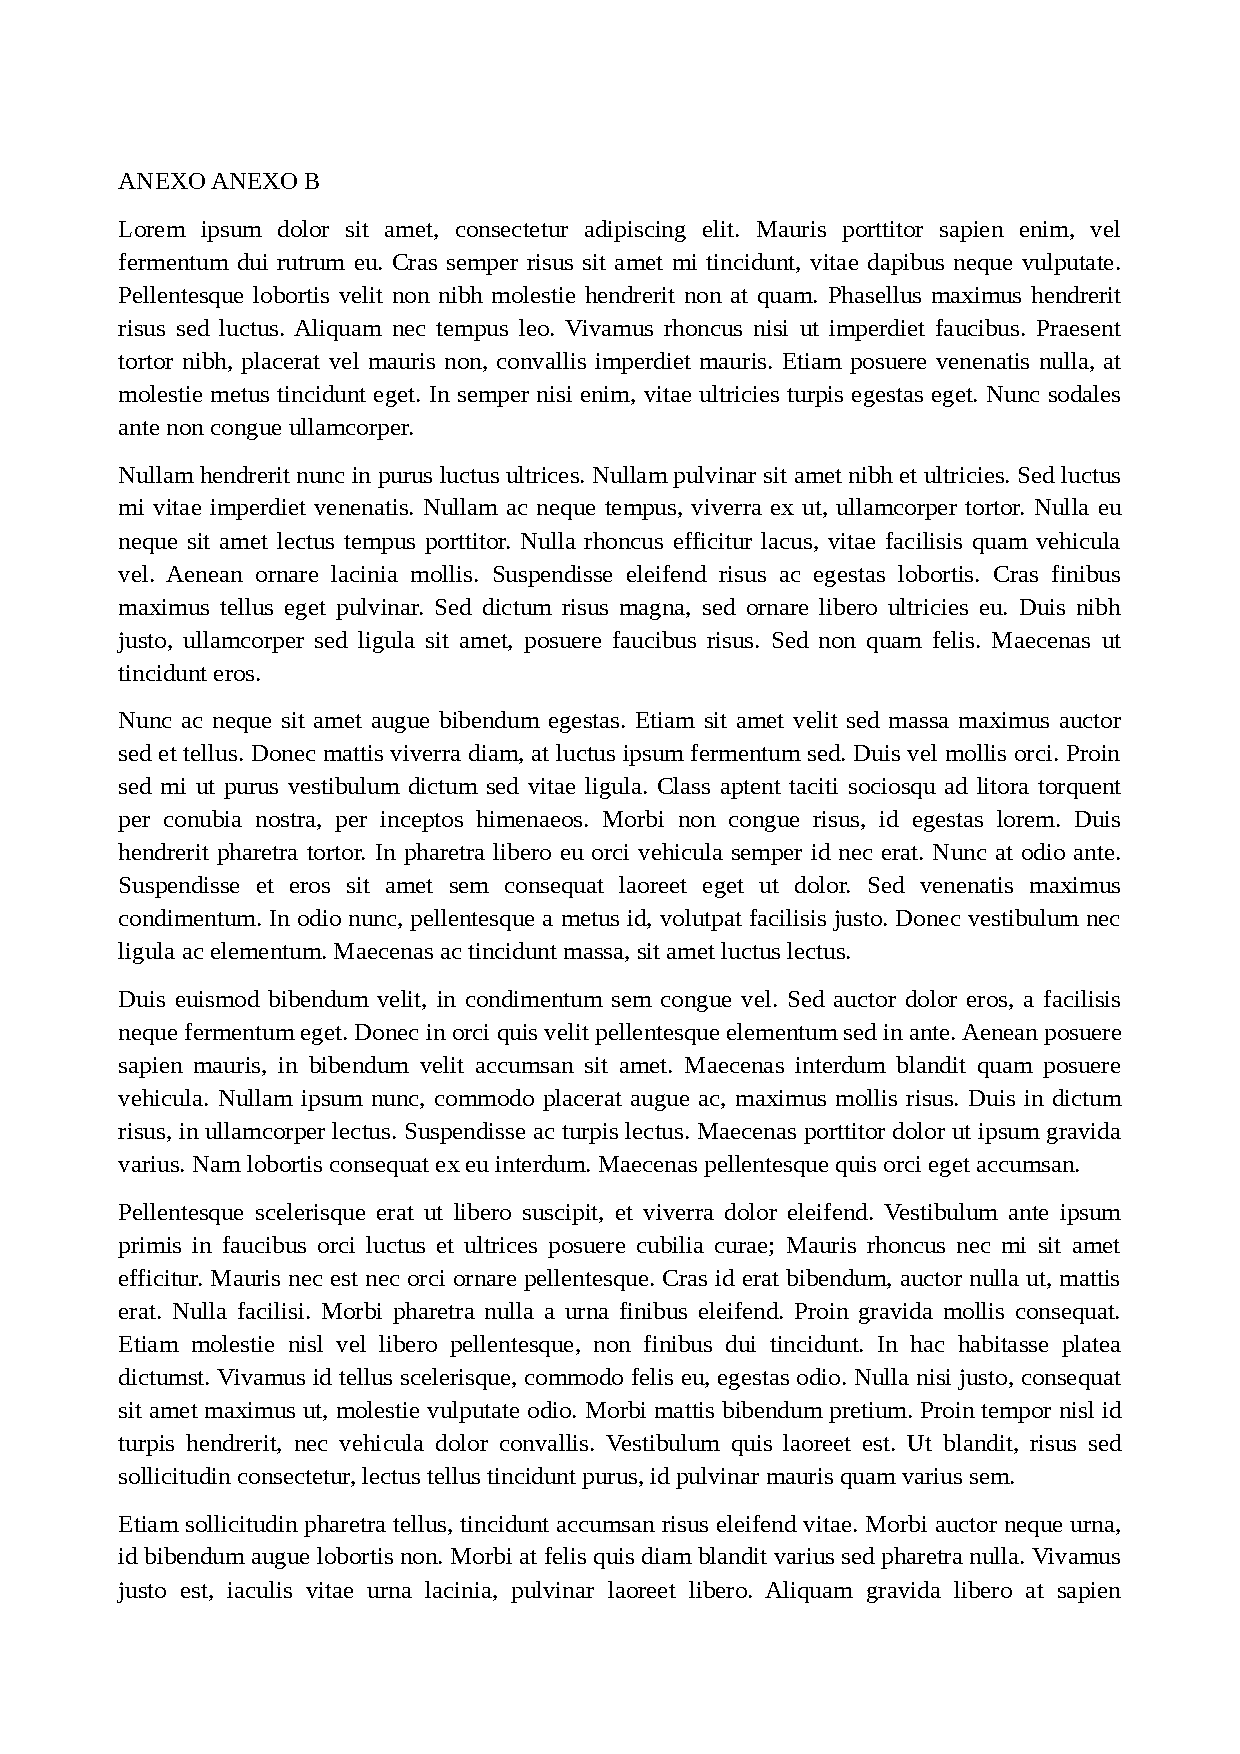
\includepdf[pages={1},scale=0.8,pagecommand=\chapter{Texto Texto Texto Texto}\label{anex:anexob}]{anexos/anexoB}
\includepdf[pages={2-},scale=0.80,pagecommand={}]{anexos/anexoB}

%coloca o identificador do anexo/apendice somente na primeira página
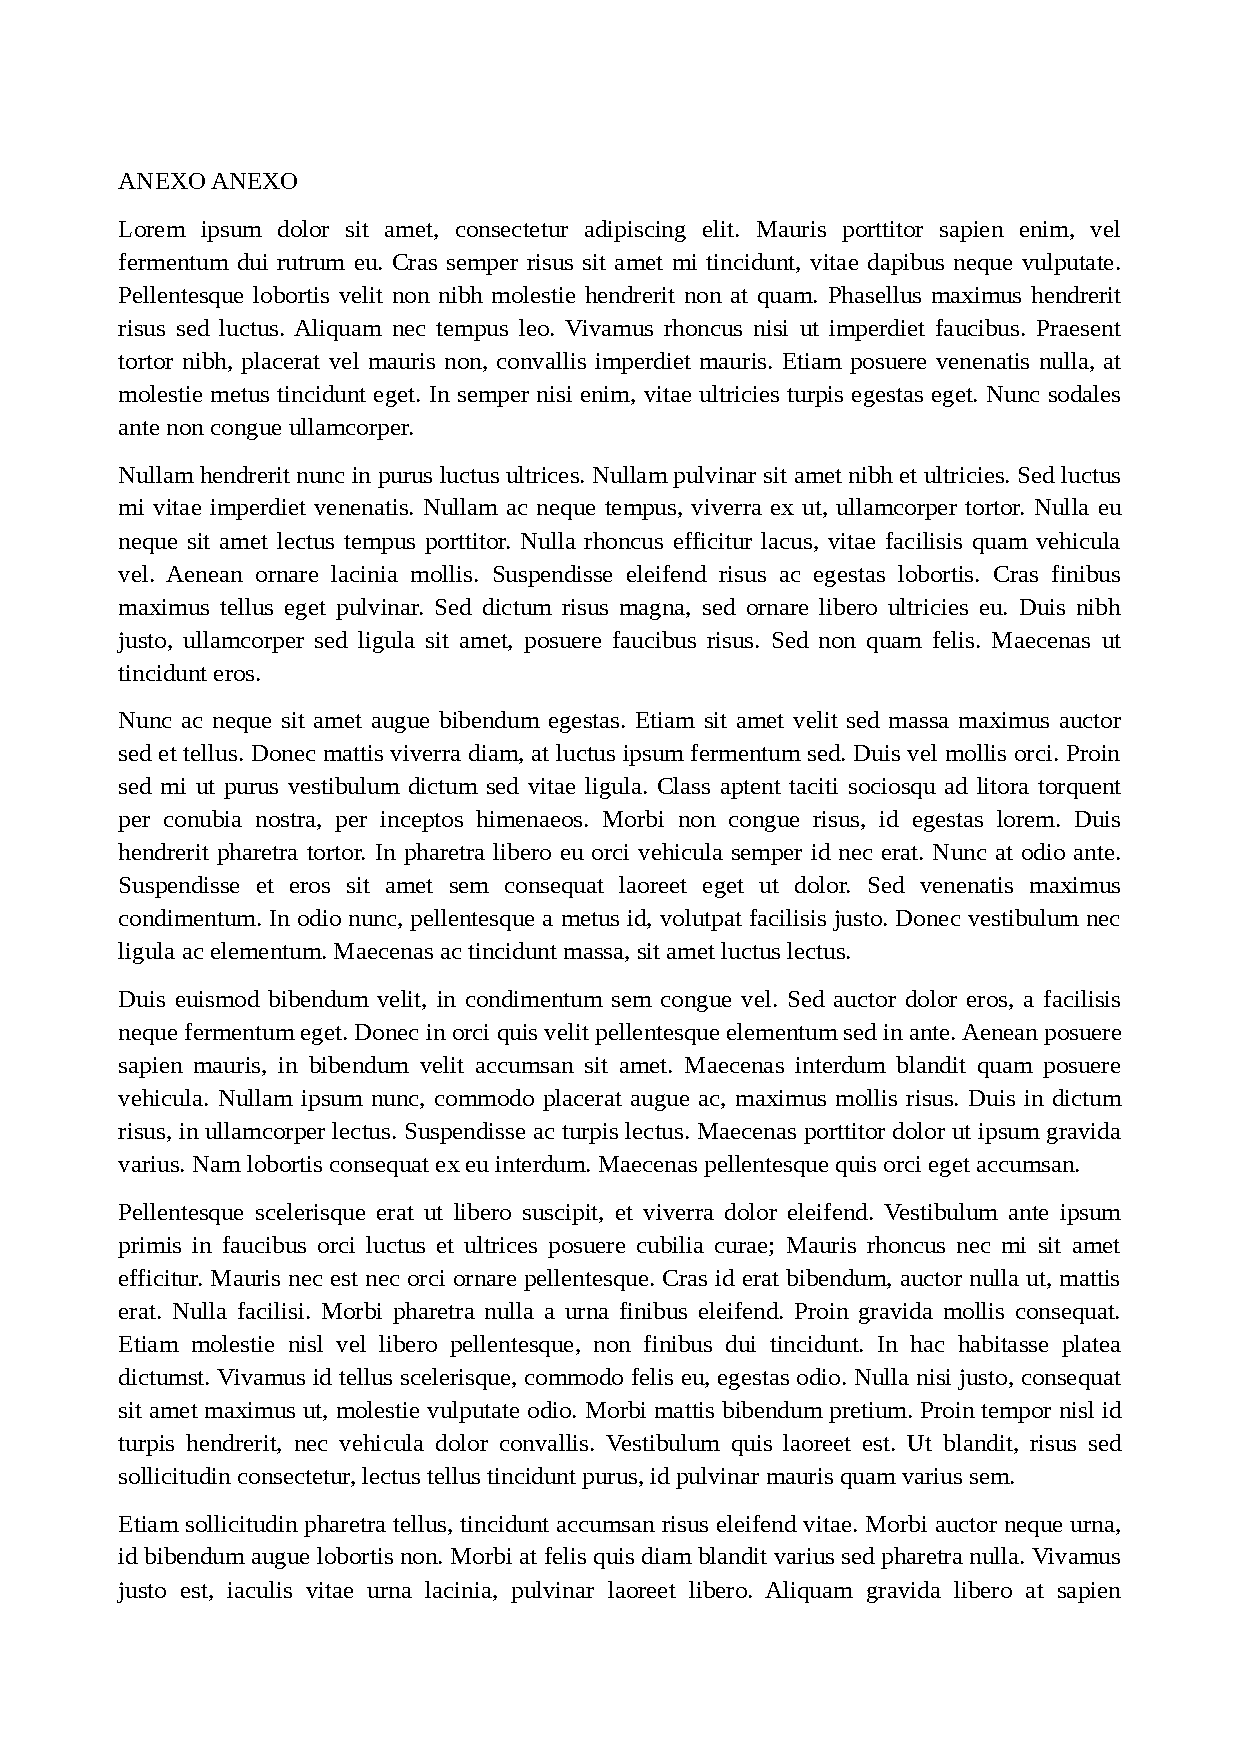
\includepdf[pages={1},scale=0.8,pagecommand=\chapter{Texto Texto Texto Texto}\label{anex:anexoa}]{anexos/anexoA}
\includepdf[pages={2-},scale=0.80,pagecommand={}]{anexos/anexoA}

\addtocontents{toc}{\endgroup}
\end{anexosenv}





\printindex


\end{document}
